% PLEASE USE THIS FILE AS A TEMPLATE
% Check file iosart2x.tex for more examples

% add. options: [seceqn,secthm,crcready]
\documentclass[sw]{iosart2x}
\usepackage{todonotes}
\usepackage{cleveref}
\usepackage{csquotes}
\usepackage{aurl}
%\usepackage{dcolumn}

%%%%%%%%%%% Put your definitions here
\newcommand{\aw}{AnthroWorks3D}
\daurl{anno}{https://annosaxfdm.de/ontology/}

%%%%%%%%%%% End of definitions

\pubyear{2023}
\volume{0}
\firstpage{1}
\lastpage{1}

\begin{document}

\begin{frontmatter}

%\pretitle{}
\title{The Anthropological Notation Ontology (ANNO): A core ontology for annotating human bones and deriving phenotypes}
\runtitle{Anthropological Notation Ontology}
%\subtitle{}

% For one author:
%\author{\inits{N.}\fnms{Name1} \snm{Surname1}\ead[label=e1]{first@somewhere.com}}
%\address{Department first, \orgname{University or Company name},
%Abbreviate US states, \cny{Country}\printead[presep={\\}]{e1}}
\todo{Autorenreihenfolge festlegen}
% Höffner, Heuschkel, Schmiedel, Penne, Fritzsch, Ludwig, Mohaupt, Labudde, Uciteli
% TODO: overleaf
% Two or more authors:
\begin{aug}
\author[B]{\inits{M.}\fnms{Marie} \snm{Heuschkel}\ead[label=e3]{marie.heuschkel@hs-mittweida.de}}
\author[A]{\inits{K.}\fnms{Konrad} \snm{Höffner}\ead[label=e1]{konrad.hoeffner@uni-leipzig.de}%
\thanks{Corresponding author. \printead{e1}.}}
\author[B]{\inits{F.}\fnms{Fabian} \snm{Schmiedel}\ead[label=e5]{a@somewhere.com}}
\author[B]{\inits{L.}\fnms{Laura} \snm{Penne}\ead[label=e8]{a@somewhere.com}}
\author[B]{\inits{H. T.}\fnms{Hanjo Tim} \snm{Fritzsch}\ead[label=e9]{c@somewhere.com}}
\author[B]{\inits{A.}\fnms{Andy} \snm{Ludwig}\ead[label=e2]{y@somewhere.com}}% Fraunhofer AISEC ?
\author[B]{\inits{M.}\fnms{Marleen} \snm{Mohaupt}\ead[label=e4]{kreuzer@hs-mittweida.de}}
\author[B]{\inits{D.}\fnms{Dirk} \snm{Labudde}\ead[label=e6]{dirk.labudde@hs-mittweida.de }}
\author[A]{\inits{A.}\fnms{Alexandr} \snm{Uciteli}\ead[label=e7]{alexander.uciteli@imise.uni-leipzig.de}}
\address[A]{Institute for Medical Informatics, Statistics and Epidemiology (IMISE), \orgname{Leipzig University},
Saxony, \cny{Germany}\printead[presep={\\}]{e1,e7}}
\address[B]{\orgname{Hochschule Mittweida},
Saxony, \cny{Germany}\printead[presep={\\}]{e2,e3,e4,e5,e6}}
\end{aug}

%\begin{review}{editor}
%\reviewer{\fnms{First} \snm{Editor}\address{\orgname{University or Company name}, \cny{Country}}}
%\reviewer{\fnms{Second} \snm{Editor}\address{\orgname{First University or Company name}, \cny{Country}
%    and \orgname{Second University or Company name}, \cny{Country}}}
%\end{review}
%\begin{review}{solicited}
%\reviewer{\fnms{First} \snm{Solicited reviewer}\address{\orgname{University or Company name}, \cny{Country}}}
%\reviewer{\snm{anonymous reviewer}}
%\end{review}
%\begin{review}{open}
%\reviewer{\fnms{First} \snm{Open Reviewer}\address{\orgname{University or Company name}, \cny{Country}}}
%\end{review}

\begin{abstract}
Anthropology relies on osteometric measurements of human bones, but ...
In this paper, first, we describe the anthropology domain.
Then, we discuss design decisions of modelling ANNO.
Next, we show how ANNO is published for the community.
Finally, we describe the integration of the ontology into \aw{}.
\end{abstract}

\begin{keyword}
\kwd{Ontology}
\kwd{Ontology development}
\kwd{Anthropology}
\end{keyword}

\end{frontmatter}

%%%%%%%%%%% The article body starts:
% TODO notes from meeting, einarbeiten:
% 3 Teile Kernmodule mit Use Cases, weitere Komponenten durch Community


\section{Introduction}\label{sec:introduction}

Data from historical, prehistoric anthropology~\citep{prehistoricanthropology}, as well as modern forensic science, allow for a comprehensive understanding of deceased individuals from different time periods---
ranging from their identity and health status to aspects of their behaviour, lifestyle, culture and even concerning the circumstances of their death~\citep{spurensuche}.
For example, anthropological methods can be used to determine an individual's biological profile thus providing key information about their sex, age, height and ancestry and any further individualising traits~\citep{bioprofile}.

The science of anthropology benefits from digitalisation in various way as digitisation processes facilitate location-independent and parallel work without the effects of wear and tear on the physical skeletal specimens, the material for investigation.
Current problems of access can be resolved, as examinations can be conducted even if the skeletal material from individuals or collectives are not present at the institution or may have already been reburied.
The allocation of researchers and research material greatly enhances the quality and extent of interdisciplinary collaborative research.
Moreover it allows for linking data of different study samples across geographical boundaries.
Data sets consolidated this way and adequately formalised enable the application of efficient data analysing methods such as data mining and textmining techniques that promote deeper insights.
Representing the anthropological domain through an ontology, such as the Anthropological Notation Ontology (ANNO) presented here, is an appropriate formalisation~\citep{aw3dunpublished}.

Apart from contextual information, most informative clues can be found directly on the bone.
As a result, anthropological work relies on human anatomy, particularly the skeletal system and further tissues of the musculoskeletal system to classify and describe and thus document bones, anatomical structures and diagnostic features within the overall framework of the skeleton in a comprehensive and transparent fashion (Quelle 5).\todo{Heuschkel unveröffentlichte Forschung}
By transferring the principle of Earth topography, it is possible to create a precise map of the human skeletal and musculoskeletal system's \enquote{terrain} (QUELLE 6).\todo{z.B. Beleg zur Topographie. KH: könnte man hier als Quelle die TA nehmen?}
Such a map contains visible anatomical surface structures as well as artificial objects such as measurement points or content-related or methodologically based classifications and boundaries.
These are unequivocally located by accurate and exhaustive definitions that in turn allow for their easy retrieval and moreover serve as a basis for the objective examination, for instance in the form of measurements(QUELLE 7).\todo{Heuschkel unveröffentlichte Forschung}
Therefore the focus of the first research stage in the development of ANNO was therefore on the creation and usage of such a map.

\section{Background}
There are various nomenclatures for the description of anatomical landmarks.
These allow a uniform classification of anatomical features and structures:

The \emph{Terminologia anatomica}~\citep{ta2} (TA) is a hierarchy of anatomical landmarks of the entire human body.
From its history, the Latin and Greek designations have emerged to allow standardization.
It is advantageous that these languages no longer show progress and are increasingly losing political power.
In TA, the order of structures follows the natural anatomy.
An anatomical landmark is identified by an individual identification number, the anatomical term, and the English term.
The identification number is critical because certain landmarks are redundant.
For example, there is the \emph{processus zygomaticus} at the \emph{os frontale} and the \emph{os temporale}.
Synonyms, like \emph{zygomatic bone} and \emph{malar bone}, are also given.
Terms included in the \emph{other} category include eponyms, which are concepts named after people, places or things.
For example, \emph{ossa digitorum pedis} (engl. \emph{phalanges of the foot}) are the small bones of the toes and are also denoted as \emph{ossa phalangea pedis} which are named after the Greek word \emph{phalanx} for a dense rectangular infantry formation.
% chapter 2: Ossa (Bones)

The \emph{Foundational Model of Anatomy} (FMA) ontology~\citep{fma} represents the physical organization of human anatomy.
%It allows the knowledge it contains to be represented in a human-understandable and machine-interpretable way.
However, it does not include Greek and Latin labels, which are frequently used by medical professionals.
Due to hypernyms 90\,\% of the terms are re-designated and only 1\,\% contain definitions.
This has a negative impact on the comprehensibility for users.

Furthermore, in both nomenclatures there is an inconsistent use of singular and plural forms, gaps in lateralized landmarks and numbered series of certain bones (e.g. costae).
In anatomy, it is also important to distinguish between the medical and anthropological viewpoints.
For example, relevant anthropological aspects such as the degree of wear of bones are not considered.
Furthermore, the articular surfaces of the individual bones are particularly important in anthropology.
Not all articular surfaces (e.g., on the ossa metatarsalia) are defined in the nomenclatures, resulting in further gaps.
In some cases, contradictions are also found in the definitions of individual landmarks.
For example, the corpus ossis pubis is placed elsewhere in some sources than in others.
Another problem is that the individual services do not synchronize and do not offer enough synonyms. % which services?
In addition, the anatomical landmarks are not visually represented and are only selectively labeled in known anatomy atlases.
However, since landmarks are three-dimensional structures, it is essential to provide a marker over the entire landmark and delineate it accurately.
The delineations must also be clearly described textually.
However, there are no standardized definitions in anatomy so far and also in the literature the information is sparse.
For example, in some sources only punctual labels are presented on a figure.
A similar situation exists with osteometric landmarks.
Standardized ones are found only on the cranium and mandible.
However, since there are measurement distances on all bones, the respective start and end points must also be defined.
These are stated differently in the literature and have a high number of synonyms.

For these reasons, it is necessary to develop uniform, textual, visual and detailed descriptive definitions for the individual landmarks, as well as to represent them in a new and clear way in an ontology.
The ontology should be easy to understand for the user.

% TODO: add rdfbones

%\url{https://bioportal.bioontology.org/ontologies/FMA}

\section{Ontological Architecture}\label{sec:architecture}
%Gesamtarchitektur, Zusammenhang zwischen GFO, ANNOdc, ANNOds, 3-Ontologien-Methode, alles mit Verweisen auf die nächsten Kapitel, vielleicht ein kleines Bild

%The development of ANNO and its integration into \aw{} follows the \emph{three ontology method}~\citep{threeontologymethod} for ontology-based software engineering:
%First, \emph{task ontology} is created as a conceptual model of \aw{}.
%Second, the General Formal Ontology (GFO)~\citep{gfo} is chosen as \emph{top-level ontology} to provide a theoretical foundation.
%Third, the \emph{domain ontology} is created that describes the domain of skeletal anatomy.
\todo{figure out how to best separate ontology and software}
The ontological architecture of ANNO consists of three interrelated layers.

\begin{enumerate}
  
  \item ANNOds (\cref{sec:domain}) is a domain-specific (ds) ontology for describing domain-specific entities to be used for annotating 
the parts of human skeleton (bones, teeth and landmarks, such as, mandible, left mandibular central secondary incisor tooth 
or mentale dexter) as well as to model their properties and relations (e.g., the distance between mentale dexter and mentale sinister) 
required to derive human phenotypes (e.g., sex or height). The ANNOds is embedded in ANNOdc 
(i.e., the ANNOds classes are subclasses of the ANNOdc classes).
  
  \item ANNOdc (\cref{sec:core}, \cref{fig:core}) is a domain-core (dc) ontology to provide the core entities of a domain, such as, inter alia, 
the general anatomical categories (\aurl{anno}{Anatomical_structure} and \aurl{anno}{Landmark}), categories for describing different characteristics of 
landmarks (\aurl{anno}{Landmark_location}, \aurl{anno}{Landmark_property} and \aurl{anno}{Landmark_line_region}) as well as 
the category \aurl{anno}{Phenotype} to model the rules for determining human phenotypes. The ANNOdc is founded by \emph{General Formal Ontology} (GFO)~\citep{gfo}.
  
  \item GFO is a top-level ontology and is used for integrating and founding the ANNO. In the current paper, we refer especially to the categories 
\enquote{Material object}, \enquote{Attributive}, \enquote{Relator} as well as the spatial entities of GFO (\cref{sec:core}, \cref{fig:gfo}).
\end{enumerate}

This architecture fits very well with the three-ontology method~\citep{threeontologymethod} on the basis of which we designed 
the \aw{} software (\cref{sec:aw}) for annotating human skeletons and determining phenotypes.
This method for developing consistent and modular software is based on the interaction of a task ontology, a domain ontology 
and a top-level ontology. In our case, the ANNOdc plays the role of a task ontology, while the ANNOds acts as a domain ontology. 
One of the advantages of the three-ontology method is that the software only needs to implement the access to entities (classes, properties) 
of the task ontology, whereas the entities of the corresponding domain ontology are processed dynamically. 
The \aw{} uses the ANNOdc as an interface to access the ANNOds entities, e.g. by listing all subclasses of a specific ANNOdc class, 
such as \aurl{anno}{Bone}, as described in \cref{sec:aw}.

% take care to prevent the problems noted by reviewer 1 in https://semantic-web-journal.net/content/modelling-digital-health-data-examode-ontology-histopathology
% TODO: ontology language, expressivity
% TODO: reuse of ontological entities
% TODO: clear validation mechanism
% TODO: top-level ontology?


\section{Description of ANNOdc}\label{sec:core}
% Definition/Beschreibung der Kern-Konzepte/Module und -Relationen mit Beispielen, GFO-Einbettung
\begin{figure}[h]
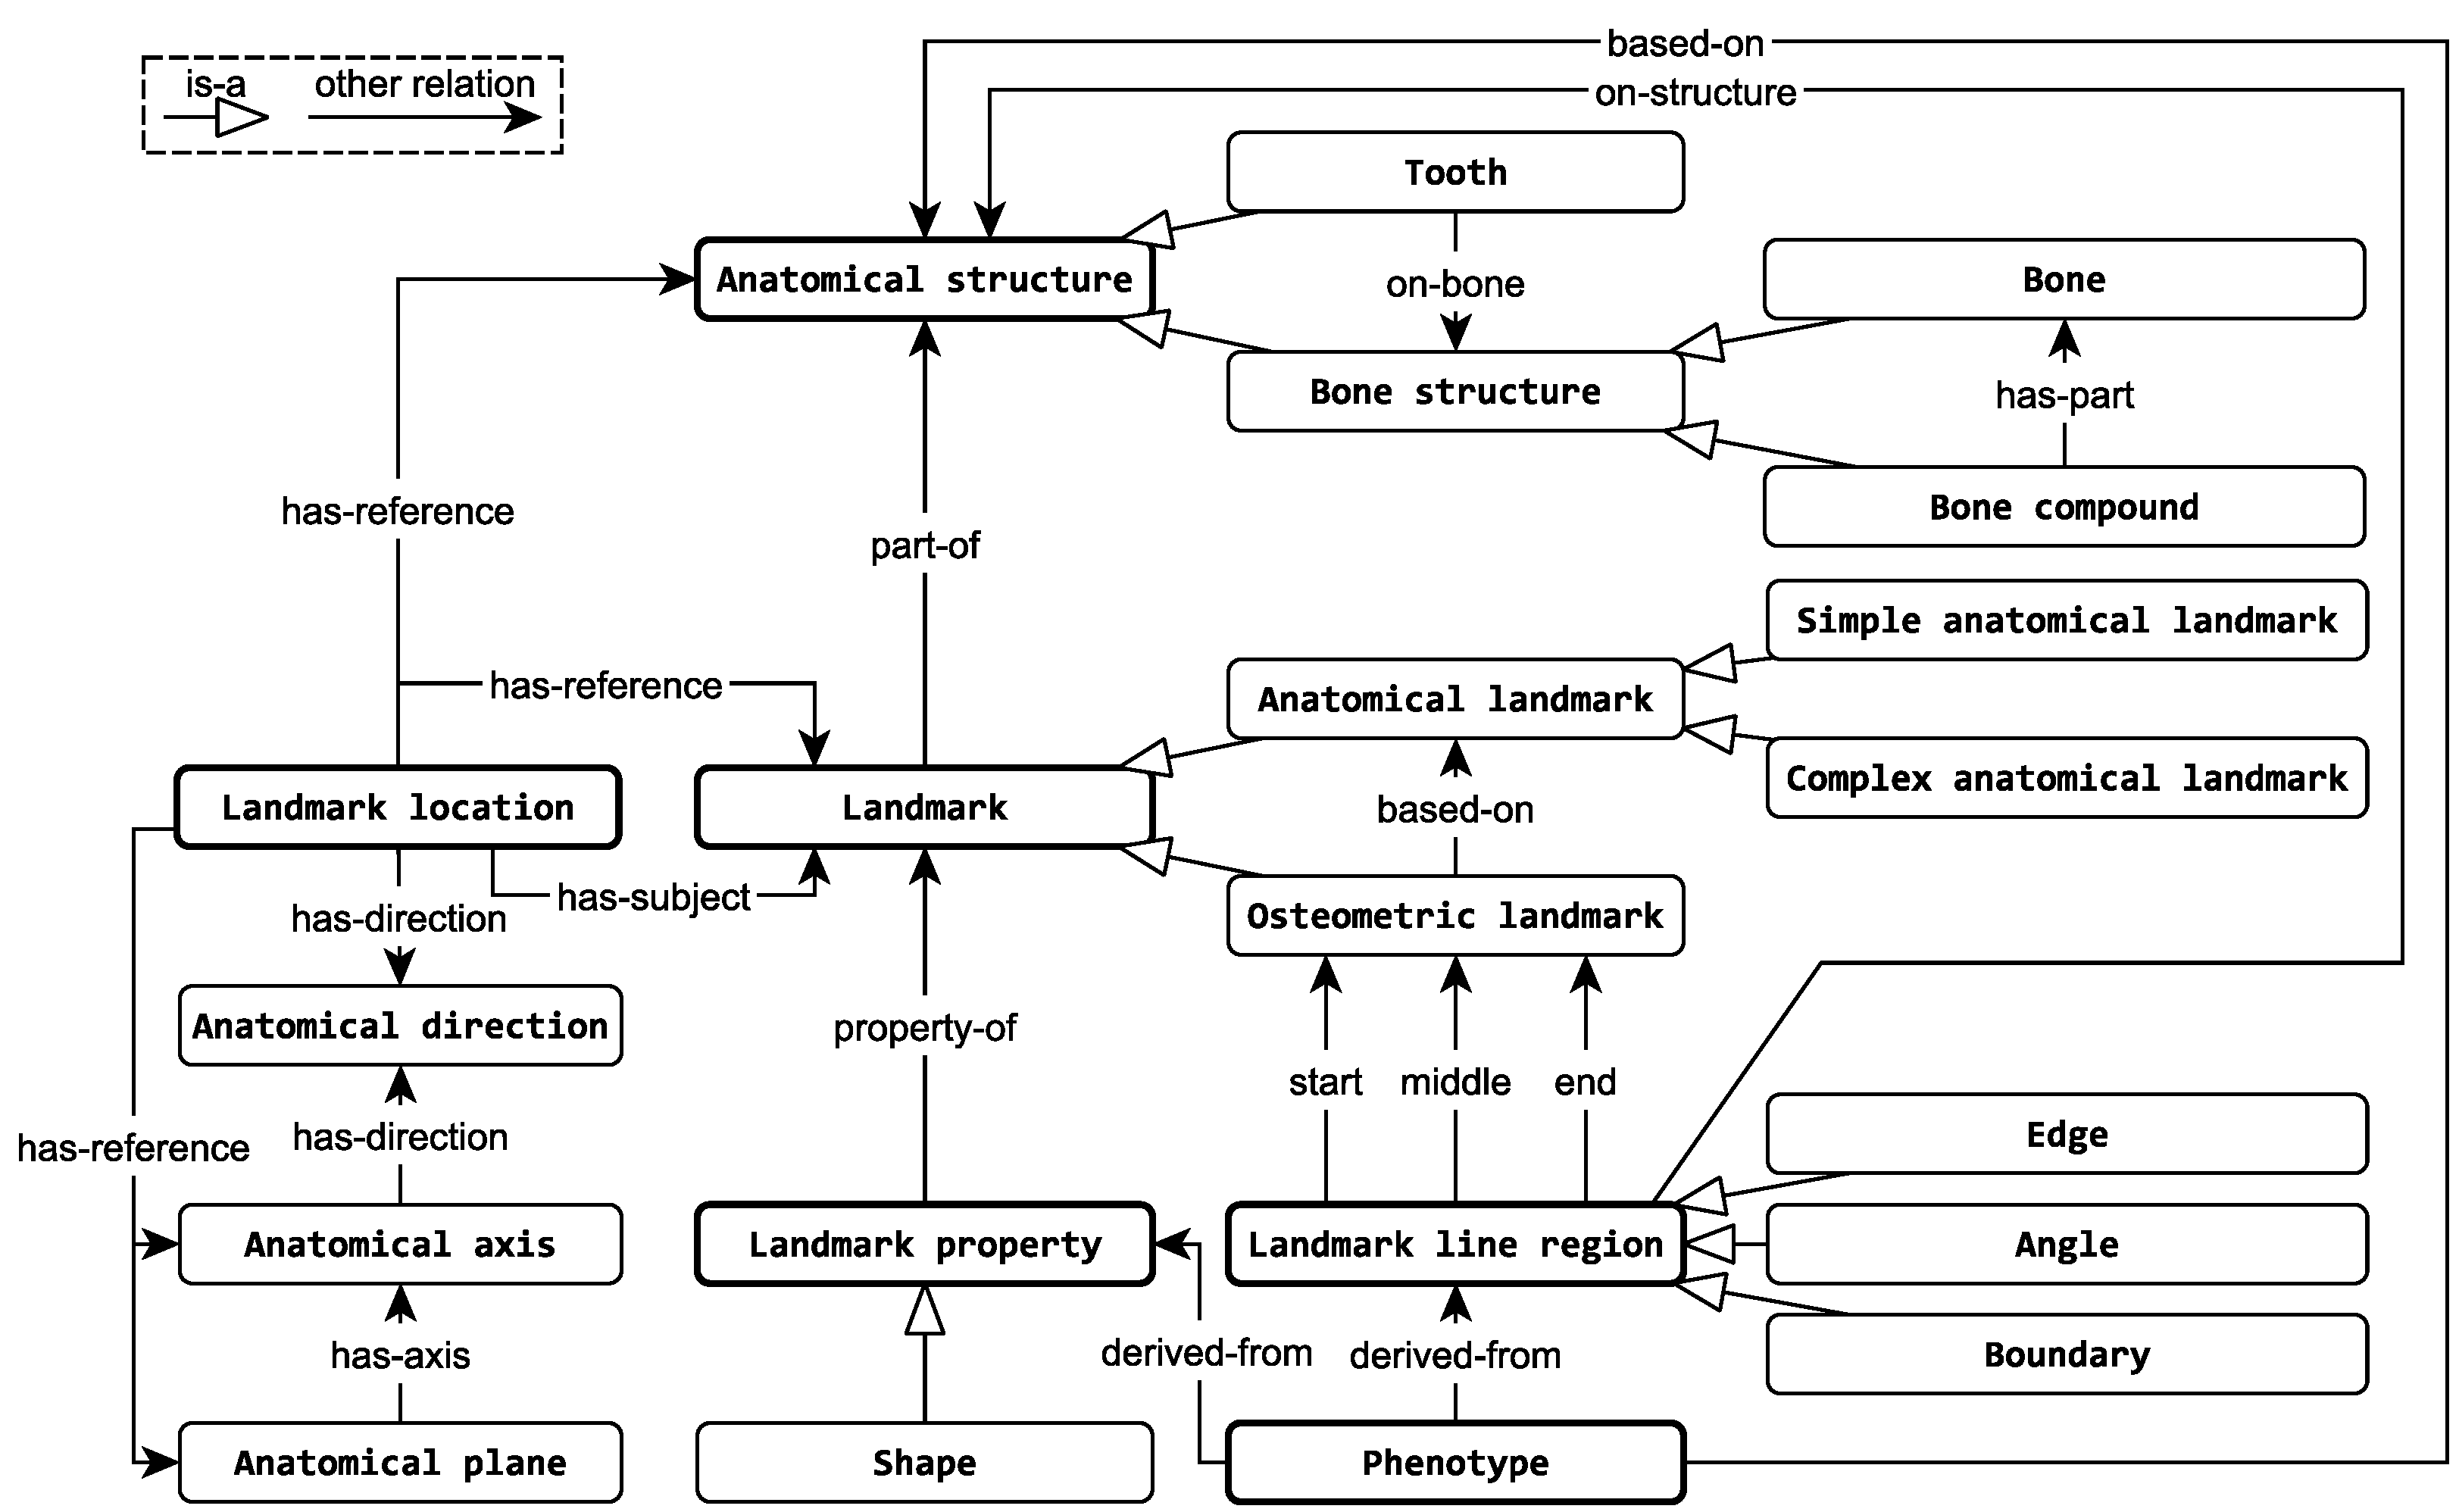
\includegraphics[width=\textwidth]{img/core.pdf}
\caption{ANNOdc ontology}\label{fig:core}
\end{figure}

\begin{figure}[h]
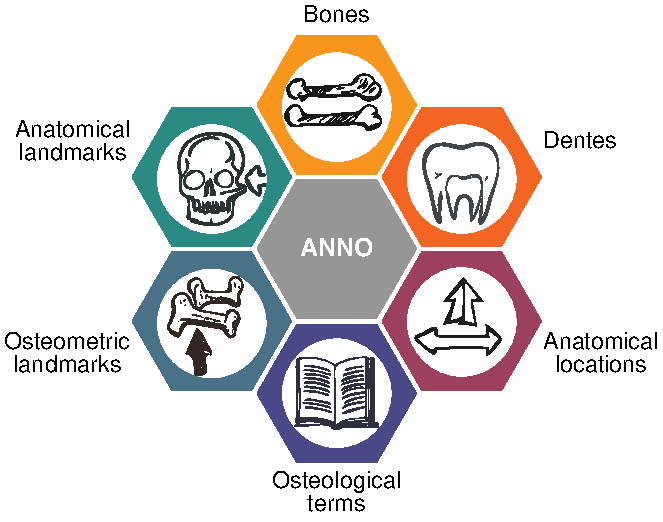
\includegraphics[width=0.3\textwidth]{img/modules.pdf}
\caption{The six modules of ANNO}\label{fig:modules}
\end{figure}
\todo{Brauchen wir \cref{fig:modules} noch oder ist sie durch \cref{fig:core} nicht mehr nötig?}

The ontology consists of the following core modules, see \cref{fig:modules}:
%For the categories, there were the following spreadsheets: bones, anatomical landmarks, osteometric landmarks, measured distances, function (separately for discriminant and regress functions), anatomical position descriptions, sources used, and osteological terminology.
\subsection{Anatomical Structures}\label{sec:bone}

In ANNO, we consider bone structures and teeth as anatomical structures relevant to the anthropology domain. 
Bone structures are divided into single bones and bone compounds consisting of further bones (has_part). 
Teeth are located on bone structures (on_bone). 

\subsection{Landmarks}\label{sec:landmark}
All landmarks are annotated with their name in singular and plural form, reference bone, synonyms, textual and visual definition, FMA and TA ID, and sources.


\paragraph{Anatomical Landmarks}
Anatomical landmarks are defined either on a bone or an anatomical compound structure.
Landmarks have properties such as shape and phenotypes are derived from those properties.

\paragraph{Osteometric Landmarks}

\subsection{Landmark Properties}

\subsection{Relative Landmark Positions}

A relative position of a landmark regarding a reference object can be described using the ANNO. 
For this, the corresponding landmark (the subject), a reference object 
(anatomical structure, anatomical axis, anatomical plane or another landmark) and, if required, an anatomical direction 
(in relation to the reference object) must be specified. If the direction was not specified, the landmark is located on the reference object.

\subsection{Landmark Line Regions and Measurements}
Landmark line regions are lines connecting or outlining landmarks (e.g., an edge between two landmarks, an angle between three landmarks 
or an outline of one or more landmarks). A landmark line region can start on one landmark and end on another, 
passing through or bordering multiple landmarks.
The landmark line regions can be measured (e.g., the length of the edge or outline and the angle degree).
Such measurements can be used to derive/determine individual phenotypes.

Measurements consist of references to sections, the start point, midpoint, end point, and short definitions.

\todo{Umschreiben von Modulen auf ANNOdc}
\subsection{Phenotypes and Functions}
Functions are categorized into sex determination and regress functions for body height estimation.
RDF is not optimized for mathematical formulas so we model those as literals.

\paragraph{Sex determination}
% auto translated from the project report, use as basis:
The sex of a specific individual within a population may be estimated using a function on skelettal measurements that is specific to this population.
Based on a threshold value, skeletons are classified into male, probably male, indifferent, probably female, and female.

\paragraph{Regress functions}
Regress functions for body height and body weight estimation.
The goal here was to cover functions for at least one European, African, American, and Asian ethnic group or population.
Names were assigned by the number included in each study, the authors, and the year of publication.
In addition, the function, reference population, aspect (e.g., discriminant function), and sample size with division by gender were noted.
In addition, for the discriminant functions, the thresholds of sex assignment, classification accuracy, and misclassification were important; for the regression functions, the error interval was important.


\subsection{Foundation of ANNO with GFO}

Anatomical structures and landmarks (as parts of anatomical structures) are material objects in the sense of the GFO because they consist of matter, have a mass and occupy space~\citep{gfospace}.
The landmark properties (such as shape) are interpreted as attributives (or qualities) in GFO~\citep{gfoarchitecture}.
These are dependent individuals that characterise other individuals (in our case, the landmarks).
The phenotype notion has already been analysed in detail within the framework of the Core Ontology of Phenotypes and defined as an individual property of an organism (such as sex or body height)~\citep{ontologicalrepresentation}.
The phenotypes are therefore also attributives in the GFO sense.
The relative position (location) of a landmark with respect to another entity is represented by GFO relators.
Relators are instances of relations, are composed of roles and link other entities together~\citep{gfocategory}.
The landmark location relator consists of three roles: subject (the landmark whose position should be described), the reference object (anatomical structure, landmark, axis or plane) and the direction (e.g., cranial or lateral).
In this way, the relative position of landmark A to landmark B (A lies lateral from B) can be described \todo{hier ein echtes Beispiel}.
We call the lines connecting landmarks in space (e.g., an edge between two landmarks or an angle between three landmarks) as well as spatial boundaries of
landmarks---landmark line regions---and associate them with line regions (one-dimensional space entities) in GFO~\citep{gfospace}.
The landmark line regions can be measured (i.e., the length of the edge or boundary and the angle degree).
Such measurements as well as the landmark properties (e.g., shape) can be used to derive/determine individual phenotypes.
The anatomical axes are also lines (line regions), while anatomical planes are surfaces (surface regions) in GFO (two-dimensional space entities).

\begin{figure}[h]
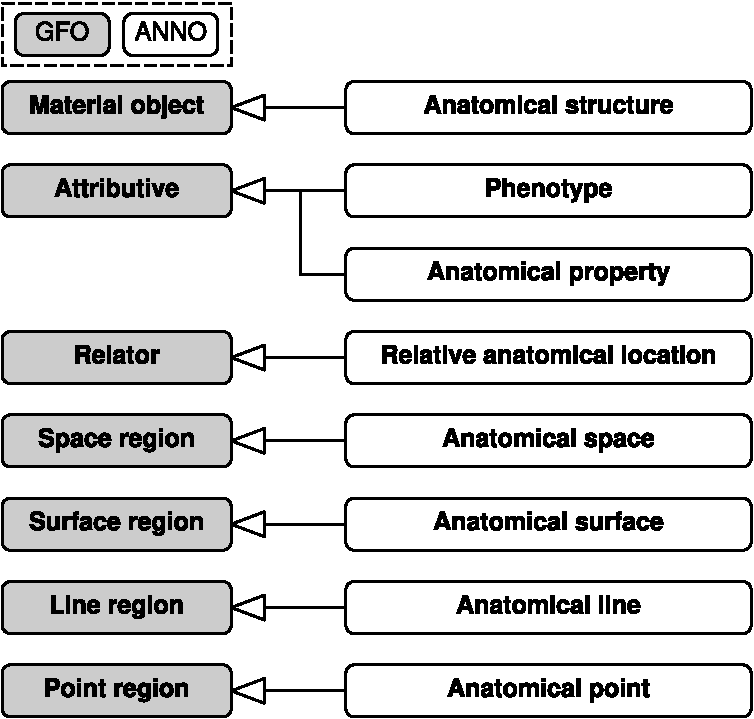
\includegraphics[width=0.6\textwidth]{img/gfo.pdf}
\caption{Integration of ANNO with the top-level GFO ontology.}\label{fig:gfo}
\end{figure}

\section{Development of ANNOds}\label{sec:domain}
% Arbeit der Domänenexperten, Tabelle, OWL-Generator
\begin{figure}[h!t]
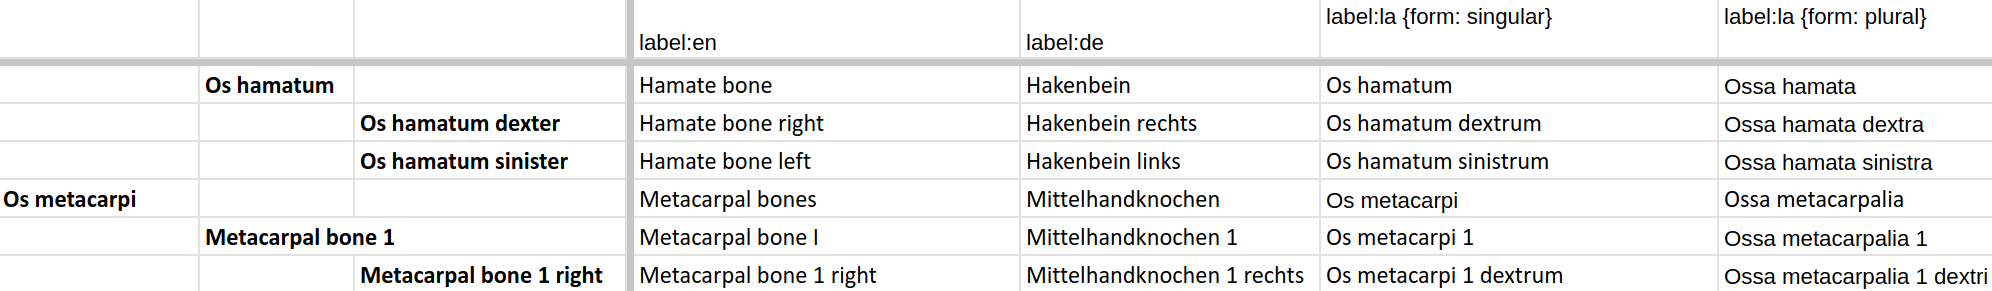
\includegraphics[width=\textwidth]{img/smog.png}
\caption{Excerpt of the spreadsheet-based input template used by the anthropologists.}\label{fig:smog}
\end{figure}

The domain experts are provided a spreadsheet-based SMOG~\citep{smog} template by the ontologists, see \cref{fig:smog}.
The spreadsheet is transformed to an OWL 2 ontology consisting of a taxonomy, annotations and some simple axioms on the basis of property restrictions.
\todo{können wir es auf OWL 2 DL eingrenzen?}

% ist das richtig übersetzt?
Sources are categorized into core, root, and occurrence sources.\todo{explain}

% Aus dem Projektbericht übersetzt
\subsection{Selection criteria}
Initially, selection criteria were made for the development of the ontology.
All bones were to be integrated.
For the individual anatomical landmarks, it was necessary to take all those that occur in the TA with the exception of anatomical variants.
However, for the cranium, the selection was reduced because the number of all ossa cranii is too high.
Overall, however, it should include those that are of anthropological relevance, i.e., contribute to navigation, localization, and identification on the bone.
Those landmarks included in the definitions of others were also to be defined.
For bones that lie on the median (e.g., mandible or sternum), bilateral landmarks were defined with side reference in each case.
For osteometric landmarks, all those already established in the core literature were to be taken.
Furthermore, those were to be taken that are relevant for meaningful measurement distances and can be annotated in \aw{}.
For measurement distances, those that are established in the bulk of the literature and core literature as well as necessary for discriminant functions and functions for body height and body weight estimation should be selected.
In addition, it also had to be integrable into \aw{}.
For the functions, those with diagnostic value were taken.
These were discriminant functions for sex determination and regression functions for body height and body weight estimation.

\subsection{Process for creating definitions and measurements}
For the definitions and measurement, a minimum amount of English-language and mostly German-language literature was compared in order to develop the definitions from their information.
Notably, Latin or ancient Greek terms were missing from the English-language literature.
The FMA also contains only English terms.
For this reason, these were also searched out with their synonyms.
Overall, the name of the landmark or survey route had to be noted in English, German, and Latin in singular and plural form, its synonyms in the three languages, the FMA and TA ID, and any information on function and delineation.
Where there were contradictions in the literature, the information was highlighted, reconciled, and logically checked.
For the osteometric landmarks, the abbreviations and their synonyms of the three languages were also provided.
Furthermore, for these as well as for the measured sections, the sources were divided into parent source, core source and occurrence source.
The parent source designates the original source of the landmark.
Under the core source, those were listed where the landmarks are listed and sampled by default.
Occurrence source represents the sources where the landmark occurs for measurements.
For redefinitions of landmarks, a meaningful Latin name had to be selected.
Requirements for this were an included position description (e.g. Punctum superioris capitis femoris as superior located point of the Caput femoris) necessary.
For this, the examination of the Latin grammar was relevant.
For the measurement sections, the type of measurement (e.g., distance measurement) and the measurement instrument were taken in addition to the name of the measurement section.
The subsequently created visual definitions were made in the different anatomical views and represented area markings for the anatomical landmarks and point markings for the osteometric ones.
\subsection{Functions}
The functions were divided into discriminant functions for sex determination and regress functions for body height and body weight estimation.
The goal here was to cover functions for at least one European, African, American, and Asian ethnicity or population.
Names were assigned by the number included in each study, the authors, and the year of publication.
In addition, the function, reference population, aspect (e.g., discriminant function), and sample size with division by gender were noted.
In addition, for the discriminant functions, the thresholds of sex assignment, classification accuracy, and misclassification were important; for the regression functions, the error interval was important.

While there are many textual sources of anthropological systematization, they do not agree in all aspects and there is not a single, formally described, standard.
ANNO links to concepts of the FMA when they exist, but structures them in a different way.

\section{Use Case: Integration into \aw{}}\label{sec:aw}
% this is based on project report but has to be rewritten: less about AW3d and more about the usage of ANNO by it
ANNO is used by \aw{}~\citep{aw3d}.
By combining user-friendly techniques of photogrammetry, insights from user experience research and knowledge from game development, a digital twin is created, which can subsequently be examined virtually.
This enables location-independent and parallel work without wear and tear on the bone.
The examination can be performed as often as desired, even if the skeletal individuals or collections are not available at the institute or have already been reburied.
It also draws its advantage when space is limited.
Thus, it requires only three SLR cameras, sufficient exposure and a computer.
The examination proceeds as follows: After photogrammetry is done and the 3D model is created, the objects are imported into the software and calibrated.
For calibration, there is an individual placeholder for each bone, which must first be selected.
Then the calibrated digital twin is placed in a placeholder skeleton.
Annotations can be made in the detailed view of each bone.
Point, line and area markings are available for selection.
Furthermore, it is possible to make measurements.
You can choose between distance, angle and circumference measurements.
After marking or measurement, an identification number is assigned to each one.
There is also a documentation about the time of the annotation as well as the name of the editor.
The marking or measurement can be classified according to certain categories (e.g. anatomical variation).
In addition, annotations are possible in a text field.
The annotations can be edited at any time afterwards, and the date of editing is recorded together with the author.
The annotations are subsequently displayed in different colors, so that overlaps can be kept apart.
A special feature of the software is the automation of measurements.
The program automatically sets pins for osteometric landmarks in a template view.
The person using the program can move these as desired.
The pins displayed have different color shades.
These differ depending on the relevance.
If the osteometric landmark is present in many measurement sections, its relevance increases and the pin appears darker.
After the pins have been roughly set, they can be refined using various views.
In the views, the individual osteometric landmarks are visible from different views, so that a fine adjustment can be made.
This is followed by the automatic measurement.
The individual values for each measurement section can be downloaded as a CSV file.
In addition, it is now possible to perform sex determinations using discriminant functions.
For this purpose, the required measurement sections can be selected.
The results are only visible in one display.
The automation allows a time saving, whereby more bones or skeletons can be examined in a shorter time.
Advantages over the previous approach are:

\begin{itemize}
\item ontology-oriented generation of placeholders/containers for objects to be imported
\item variable properties for different bone elements and bone types
\item hierarchy for orientation within an examination project according to the ontology tree
\item categorization of measurements and markers according to specifications from the ontology
\item generation of input forms based on the specified properties and bone types
\item automatic generation of measurements
\end{itemize}

%\subsection{}\label{s1.1}

\section{Conclusion and Future Work}
% Conclusion

% Basiert auf dem Fazit aus dem Projektbericht
ANNO introduces uniform definitions for the anatomical landmarks of the human skeletal system as well as osteometric landmarks, measurement distances and functions.
basis for anthropological work
The ontology is interlinked with ... and includes sources for all external definitions.
The ontology is used in \aw{} in place of an old, hard-coded format, which saves development time, separates annotation file compatibility from software versions, eases annotation through hierarchical browsing and increases interoperability.
% following two sentences are machine translated, improve and rewrite
It provides a basis for future training of ontologists, knowledge managers, further research activities and specialization opportunities in this field.
Furthermore, there is interest of the results in forensic, historical and prehistoric anthropology, pathology and medicine as well as in the field of computer science and especially medical informatics.
%Moreover, the ontology can be extended.

ANNO is published on \url{https://ols.imise.uni-leipzig.de} as well as \url{https://annosaxfdm.de/ontology/}.
TODO: Bereitstellung der Ontologie für die Community (OLS etc.).

% Future Work
can be extended with osteological terms of description
Arten von Erhebungen, Öffnungen, ...
anthropologische ebene draufmodellieren zb form
an anthropological landmark can have different anthropological properties

04-06 notizen
anschlussprojekte erweiterung
selbst wenn man nur einen einzelnen knöchel beschreibt wird dieser zuerst in das gesamte skelett
in der ebene zb lateral positioniert
könnte relation bestehen zwischen knochen
4 referenzpunkttypen
eine landmarke kann auf einer ebene liegen aber nicht auf einer achse, da sie keine ausdehnung hat
zb median sagital achse
Richtung vom reference point aus
location is eigenschaft der landmarke

%\begin{figure}[t]
%\includegraphics{}
%\caption{Figure caption.}\label{f1}
%\end{figure}

%\begin{table*}
%\caption{} \label{t1}
%\begin{tabular}{lll}
%\hline
%&&\\
%&&\\
%\hline
%\end{tabular}
%\end{table*}

\begin{figure}[h]
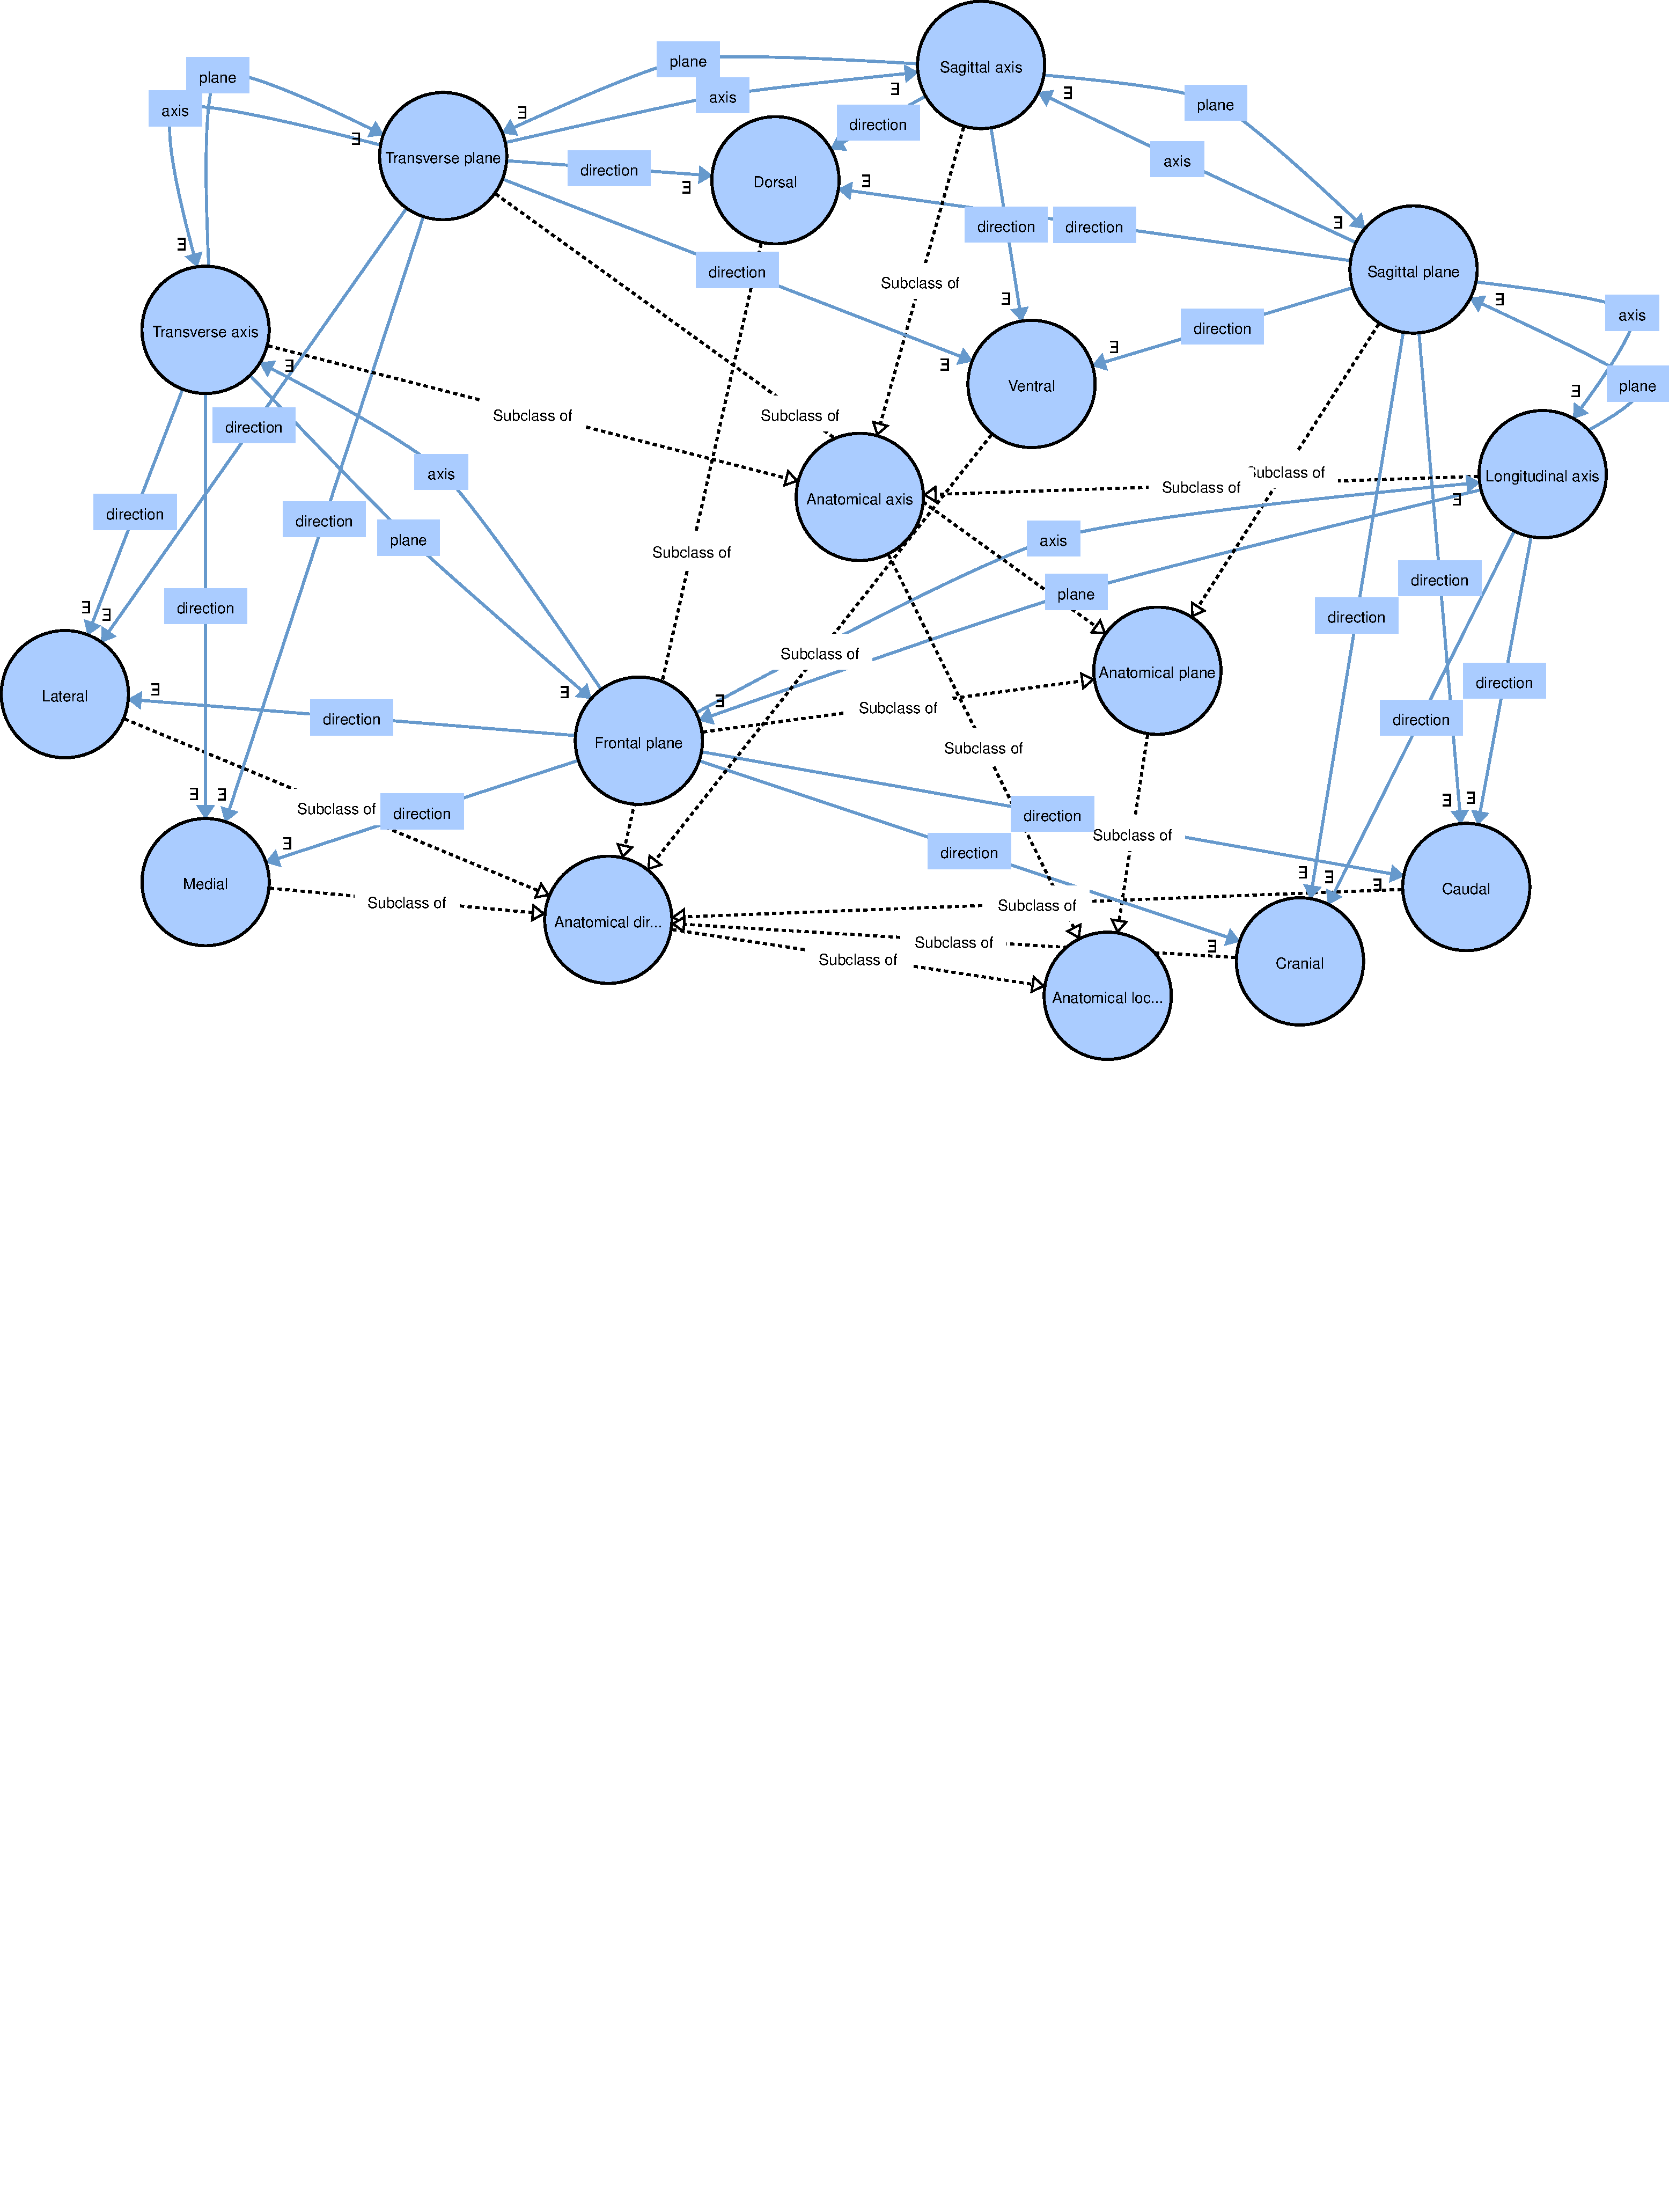
\includegraphics[width=\textwidth]{img/axisplane.pdf}
\caption{Anatomical axes and planes}\label{fig:axisplane}
\end{figure}

\begin{ack}
\noindent\begin{minipage}{0.90\textwidth}
The ANNO project is co-financed from tax funds based on the budget passed by the Parliament of the Free State of Saxony.
\end{minipage}%
\hfill%
\begin{minipage}{0.04\textwidth}\raggedleft

\includegraphics[width=\textwidth]{img/saxony.pdf}
\end{minipage}
\end{ack}

\nocite{*}
\bibliographystyle{ios1}
\bibliography{anno}
\end{document}
